\documentclass[../relazione.tex]{subfiles}

\begin{document}
\section{Progettazione}
	In seguito sono riportate in forma di elenco tutte le scelte progettuali effettuate durante lo sviluppo del progetto che il gruppo ha ritenuto degne di nota, suddivise per ambito di interesse: \texttt{XHTML}, \texttt{CSS}, \texttt{Perl/CGI}, \texttt{Javascript}, \texttt{XML} e \texttt{XMLSchema}.\\
	Tutte le scelte che riguardano puramente la parte mobile sono state riportante a parte nella sezione 5.6 \textit{Mobile} del presente documento.
	\subsection{XHTML}
	\begin{itemize}
		\item Il logo del sito è stato realizzato con una \texttt{background-image} sfruttando la tecnica di \textit{image replacement} affinché possa costituire informazione per il motore di ricerca.
		\item Nella parte pubblica del sito, il \texttt{path} svolge sia funzione di breadcrumb che di titolo della pagina: avendo un solo livello profondità, abbiamo ritenuto non necessario il breadcrumb all'interno della parte pubblica del sito.
		\item Per indicare al motore di ricerca l'importanza dei termini caratteristici del ristorante e della cucina giapponese è stato usato \texttt{strong}: questa è un'operazione di SEO (\textit{Search Engine Optimization}).
		\item La struttura di ogni pagina è stata pensata per evidenziare le informazioni che si ritengono più importanti per un utente che naviga su un sito di ristorazione. Quindi si è deciso di tenere in alto e visibile in maniera chiara in ogni pagina della parte pubblica del sito i seguenti elementi:
		\begin{itemize}
			\item il \textit{luogo} dove si trova il ristorante, che è un'ancora a \texttt{dove-siamo.html}: una pagina che presenta informazioni più dettagliate sulla posizione del ristorante
			\item il \textit{numero di telefono}, che è un'ancora alla funzione di inizio della telefonata (\texttt{tel:})
		\end{itemize}
		\item Nella pagina \texttt{index.html} sono stati messi in evidenza l'\textit{orario}, le \textit{informazioni generali} riguardo il ristorante e la possibilità di usufruire del servizio di \textit{take away}.
		\item Per fidelizzare il cliente, nella pagina \texttt{chi-siamo.html} mostriamo le personalità principali che gestiscono l'attività, come il proprietario del ristorante e i cuochi, raccontando un sunto del loro curriculum o le loro esperienza passate nel campo della ristorazione.
		\item Nella pagina \texttt{dove-siamo.html} è presente una breve descrizione testuale di dove si trova il ristorante accompagnata da un'immagine che ne indica la posizione rispetto ai vicini punti di interesse. Per rendere accessibile l'immagine a chi utilizza uno screen reader è stato utilizzato l'attributo \texttt{longdesc} che associa una descrizione testuale dettagliata (definita nel file \texttt{indicazioni.txt}) all'immagine. Oltre a questo, è presente un link a Google Maps per agevolare l'utente nella ricerca di indicazioni precise per raggiungere il ristorante: nel caso in cui stia navigando da un dispositivo mobile ed abbia l'applicazione di Google Maps installata, verrà automaticamente lanciata l'applicazione.
		\item Nella pagina \texttt{curiosita.html} abbiamo inserito una serie di curiosità sulla cucina giapponese per far conoscere all'utente un po' della sua storia.
		\item Tutti i nomi delle pietanze nella pagina \texttt{menu.cgi} sono inseriti in un tag \texttt{strong} per indicarne l'importanza al motore di ricerca: questa è un'operazione di SEO (\textit{Search Engine Optimization}).
		\item L'area amministratore permette di aggiungere, modificare o rimuovere pietanze o bevande dal menù.
	\end{itemize}
	\subsection{CSS}
	\begin{itemize}
		\item Si è cercato di utilizzare meno colori possibili.
		\item Si è scelto di utilizzare i colori di bandiera del ristorante, ricavati dal logo fornitoci dal proprietario del ristorante.
		\item Tali colori sono stati scelti antagonisti, per venire incontro a utenti con problemi di colorblindness ed aumentando così l'accessibilità del sito.
		\item Lo sfondo in legno dell'intero sito web vuole ricordare la stuoia usata nel processo di creazione del sushi e, più in generale, lo stile nipponico.
	\end{itemize}
	\subsection{Perl/CGI}
	\begin{itemize}
		\item 
	\end{itemize}
	\subsection{Javascript}
	\begin{itemize}
		\item Il menu del sito (chiamato d'ora in poi anche \texttt{nav}) è inizialmente visibile, così se \texttt{Javascript} non è attivo il sito ha una degradazione elegante.
		\item Se invece \texttt{Javascript} è attivo e la navigazione viene effettuata da mobile, allora il \texttt{nav} viene nascosto e rimane accessibile dall'apposita \texttt{icon hamburger}.
		\item È presente il controllo tramite \texttt{Javascript} dei dati inseriti nei campi delle form, per segnalare eventuali errori all'utente in maniera immediata, senza attendere una risposta del server.
		\item Nella pagina \texttt{menu.cgi} e \texttt{private-menu.cgi}, il menù è diviso in categorie inizialmente chiuse per diminuire la lunghezza della pagina e dare all'utente una visione generale delle categorie di pietanze e bevande presenti nel menù.
		\item Nel caso in cui il \texttt{Javascript} non sia attivo, il menù verrà mostrato per intero, ma viene aggiunta una funzionalità di ricerca veloce (in alto nella pagina) e, alla fine di ogni categoria, un'ancora per tornare all'inizio della pagina.
	\end{itemize}
	\subsection{XML e XMLSchema}
	\begin{itemize}
		\item 
	\end{itemize}
	\subsection{Mobile}
	Una grossa fetta di utenza del sito è composta dai ragazzi più giovani, come dimostrato dall'analisi presente alla sezione 3 \textit{Analisi dell'utenza} del presente documento.
	Per questo motivo il gruppo ha deciso di definire lo stile del sito anche per i dispositivi mobile, tenendo conto che la maggior parte degli accessi al sito da parte di ragazzi giovani verrà effettuata da smartphone o tablet.\\
	Di seguito sono riportate le scelte progettuali effettuate durante lo sviluppo del progetto che il gruppo ha ritenuto degne di nota per quanto riguarda la parte mobile del sito.
	\begin{itemize}
		\item È stata usata la \texttt{hamburger icon} come simbolo del menu del sito (\texttt{nav}), ritenuta adeguata in quanto è ormai una consuetudine per gli utenti associare ad essa il menu del sito.
		\item Per agevolare la visita del sito e rendere più piacevole l'esperienza dell'utente, abbiamo dato all'utente la possibilità di aprire e chiudere il \texttt{nav}: per far ciò è stata utilizzata una funzione \texttt{Javascript} che mostra e nasconde il \texttt{nav} attraverso la \texttt{hamburger icon}.
		\item Abbiamo convenuto che la parte mobile sia dedicata interamente agli utenti esterni, quindi abbiamo impedito l'accesso all'area amministratore da mobile: esso è permesso solo da desktop.
		\item Il sito è stato testato sui seguenti browser mobile: Google Chrome, Safari.
	\end{itemize}
	\begin{figure}[H]
		\centering
		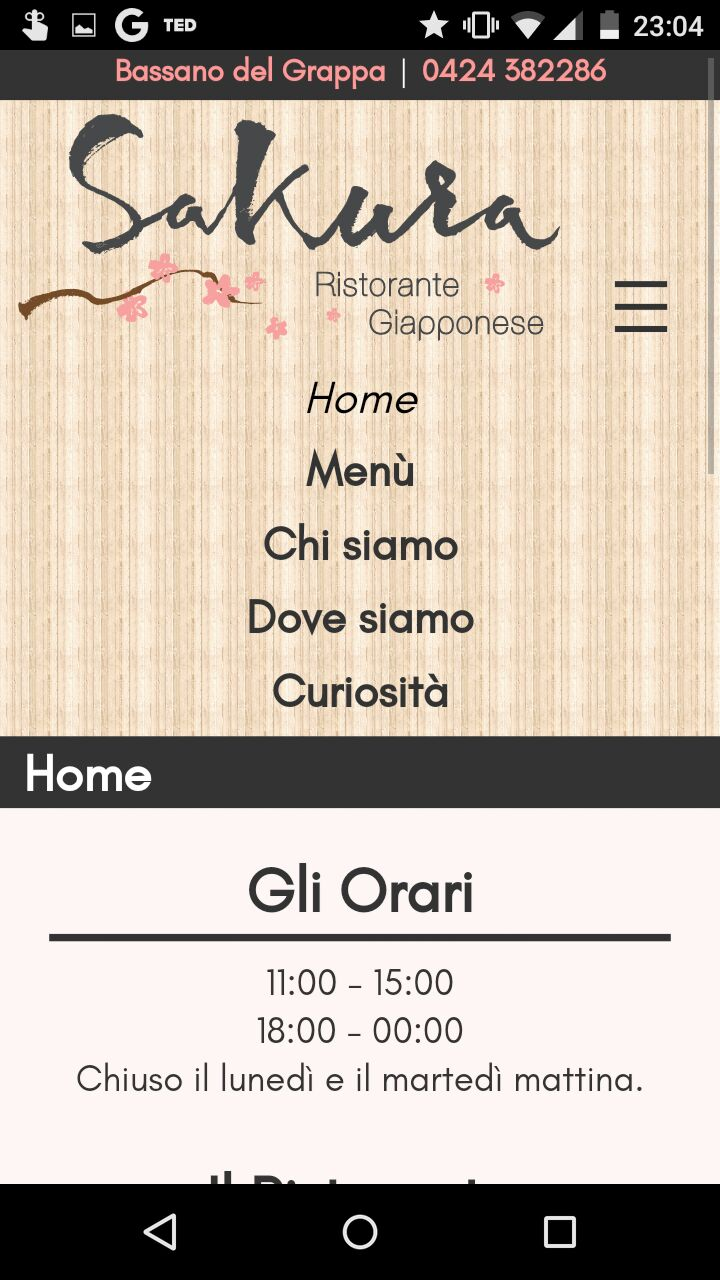
\includegraphics[scale=0.2]{images/mobile2}
		\caption{Esempio di pagina vista da dispositivo mobile con menu a tendina aperto}
		\label{fig:Esempio di pagina vista da dispositivo mobile con menu a tendina aperto}
	\end{figure}
\end{document}